\subsection{Cálculos teóricos}
\subsubsection{Esboço da derivada e integral de cada uma das formas de onda}

Usando o \textsc{matlab} podemos expressar cada uma das formas de onda muito facilmente. Usando uma frequência de $f=10 \,Hz$, temos o seguinte código para onda senoidal


\lstinputlisting{codigos/plot_onda.m}


\begin{figure}[H]
    \centering
    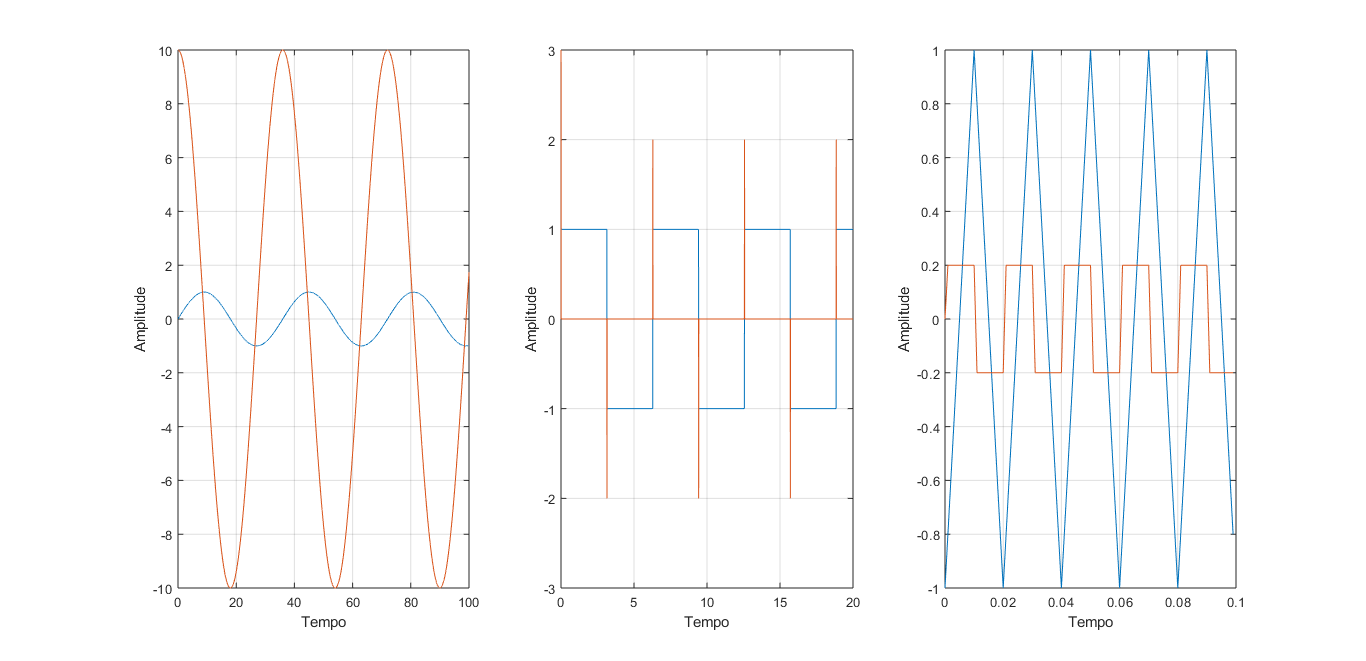
\includegraphics[width=1\textwidth]{imagens/plot_waves.png}
    \caption{Onda senoidal e sua derivada}
    \label{fig:onda_sin}
\end{figure}

% ---------------------------------------------------------------------

\subsubsection{Expressão em Laplace de $V_{out}(t)$ em função de $V_{in}$ do amplificador-diferenciador com $R_c=0$} 

Usando a expressão dada pela equação \ref{eqn:diff}, podemos escrever a transformada de Laplace como:


\begin{gather*}
	V_{out}(s) = -RC sV_{in}(s)
	\Longrightarrow \dfrac{V_{out}(s)}{V_{in}(s)} = H(s) = -RCs
\end{gather*}

Para analisar essa função de transferência, podemos plotar o diagrama de bode e observar seu comportamento.

\begin{figure}[H]
	\centering
	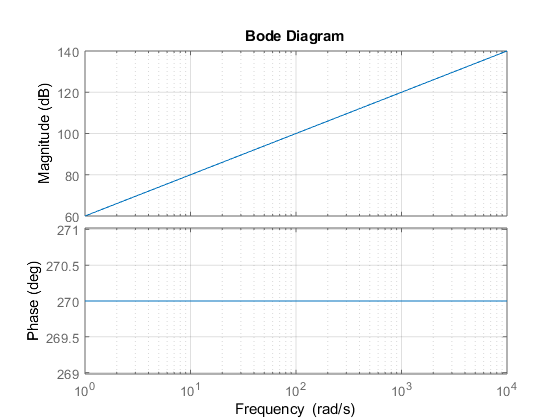
\includegraphics[width=.4\textwidth]{imagens/bode_plot.png}
	\caption{Diagrama de Bode da função de transferência}
	\label{fig: bode_dia}
\end{figure}

Considerando $R=1 k\Omega$ e $C=1F$, a função de transferência nos da um zero em 0 e um valor constante inicial de $20\cdot log(1000) = 60$. Como temos apenas um zero, a magnitude irá aumentar $ 20dB$ por década. Isso significa que quanto mais aumentarmos a frequência, maior será a amplitude da onda observada.
O que implica que, aumentando a tensão rapidamente, podemos chegar a um estado de saturação do Amp Op a partir de frequências muito pequenas dependendo do dimensionamento dos componentes.

\subsubsection{Expressão em Laplace de $V_{out}(t)$ em função de $V_{in}$ da Fig. \ref{fig:diferenciador} com $R_c>0$}

A forma mais simples de deteminar a função de transferência é transformando os componentes em impedâncias, como na figura abaixo:


\begin{figure}[H]

	\centering
	
    \begin{circuitikz}[line width = .5pt, scale = .8, transform shape]
        \draw
            (0,0) node [op amp] (opamp) {}
		
		(opamp.-) to [short] ($(opamp.-)+(0,1)$) to [generic, l_= $Z_2$]  ($(opamp.-)+(-2.8,1)$) to [generic, l_=$Z_1$] ($(opamp.-)+(-4,1)$) to [short, -o] ($(opamp.-)+(-5,1)$) node [left]{$V_{in}(t)$}
		(opamp.-) to [short, -*] ($(opamp.-)+(0,1)$)
		to [generic, l^=$Z_3$] ($(opamp.-)+(2,1)$) -| (opamp.out) to [short, *-o] ($(opamp.out)+(1,0)$)
		node [right] {$V_{out}(t)$}

		(opamp.+) to [short] ($(opamp.+)+(0,-1)$) node [ground]{}		
		;
		\draw ($(opamp.-)+(0,1)$)node[above] {A};
        
    \end{circuitikz}
    \caption{Circuito amplificador-diferenciador}
    \label{fig:diferenciador_imp}
\end{figure}


Fazendo as equações a partir da lei de Kirchhoff, obtemos:
\begin{gather*}
	\dfrac{V_A - V_{in}}{Z_1 + Z_2} + \dfrac{V_A -V_{out}}{Z_3} = 0
	\Longrightarrow\dfrac{V_{out}}{Z_3} = \dfrac{-V_{in}}{Z_1 + Z_2}\\
	\dfrac{V_{out}(s)}{V_{in}(s)} = H(s) = \dfrac{Z_3}{Z_1 + Z_2} 
\end{gather*}
Substituindo $Z_1 = R_c, \, Z_2 = \dfrac{1}{sC}, \, Z_3 = R$, temos
\begin{equation}
	H(s) = \dfrac{-RsC}{R_c sC + 1}
\end{equation}

Com uma rápida inspeção, podemos notar que a função tem um zero e um polo. O que significa que, em alguma frequência, o circuito irá se estabilizar. 

\begin{figure}[H]
	\centering
	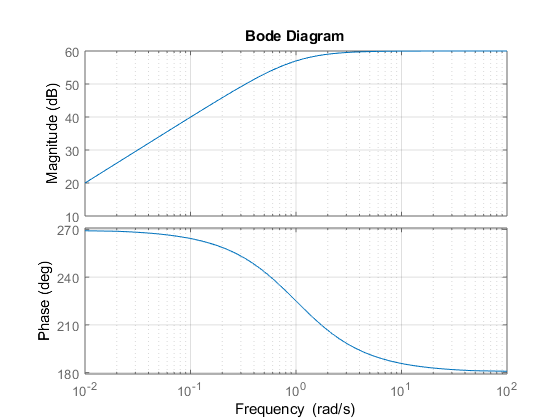
\includegraphics[width = .4\textwidth]{imagens/bode_plot_w_rc.png}
	\caption{Gráfico de Bode com $R_c>0$.}
\end{figure}

Observando o diagrama de bode dessa função de transferência com $R_c = 1\Omega, \, R = 1k\Omega \, e \, C = 1F$, podemos perceber que o circuito se estabiliza a partir das frequências de 1 kHz, com um ganho de 60 dB constantes. 

\subsubsection{Expressão para $V_{out}(t)$ da Fig. 2.2, em função de $V_{in}(t)$ e assumindo $R\rightarrow\infty$}

Utilizamos da equação \ref{eqn:int} para gerar a função no domínio da frequência a partir da Transformada de Laplace. Assim, temos
\begin{gather*}
	V_o(s) 	= -\dfrac{1}{RC} \cdot \dfrac{1}{s} \cdot V_{in}(s)
	\Longrightarrow \dfrac{V_o(s)}{V_{in}(s)} = -\dfrac{1}{RCs} 
\end{gather*}

\begin{equation}
	H(s)	=	 -\dfrac{1}{RCs}
\end{equation}

Podemos observar que a função possui apenas um polo. Dessa forma, dada uma frequência baixa, a tensão no capacitor pode ser superabundante a fim de danifica-lo. O gráfico de Bode abaixo ilustra bem a preocupação.

\begin{figure}[H]
	\centering
	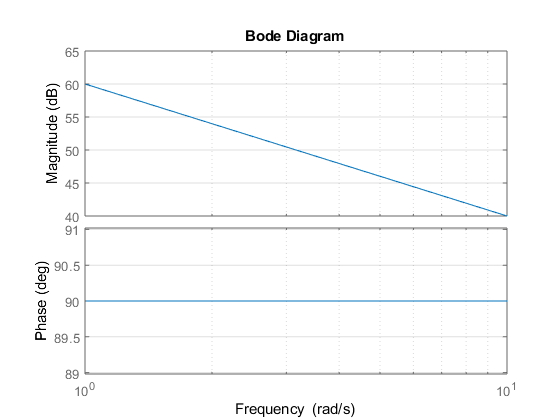
\includegraphics[width=.4\textwidth]{imagens/bode_plot_fig2_2_infty.png}
	\caption{Diagrama de Bode para $R_0 \rightarrow \infty$ }
	\label{fig: bode_2.2_rinf}
\end{figure}


Considerando C = $1\mu F$ e R = $1k\Omega$, temos uma ganho de 20 dB por década se decrescermos a frequência. Isso gera um risco para o capacitor ligado diretamente a saída do Amp Op. Por esse motivo, nunca devemos fazer $R_0 \rightarrow \infty$.

\subsubsection{Expressões para $V_{out}(t)$ da Fig. \ref{fig:integrador} em função de $V_{in}(t)$ assumindo $R_0$ finito}

Ilustrando o circuito no domínio da frequência, podemos realizar os cálculos usando apenas impedâncias, como ilustrado na figura \ref{fig:integrador_w_z}. Utilizando a Lei de Kirchhoff podemos obter a seguinte expressão.

\begin{gather*}
	\dfrac{V_A - V_{in}}{Z_1} + \dfrac{V_A-V_o}{Z_3} + \dfrac{V_A - V_o}{Z_2} = 0
	\Longrightarrow \dfrac{V_o(Z_3+Z_2)}{Z_3Z_2} = -\dfrac{V_{in}}{Z_1}
	\Longrightarrow \dfrac{V_o (s)}{V_{in}(s)} = H(s) = -\dfrac{Z_3Z_2}{(Z_3 +  Z_2)Z_1}
\end{gather*}

Substituindo $Z_3 = R_0, \, Z_2 = \frac{1}{sC}, \, e \, Z_1 = R$ e arranjando os termos, temos

\begin{equation}
	H(s) = -\dfrac{R_0}{R} \cdot\dfrac{1}{sR_0C + 1}
\end{equation}

\begin{figure}[H]
\centering
\begin{circuitikz}[line width = .5pt, scale = .8, transform shape]

\draw

	(0,0) node [op amp] (opamp) {}
	
	($(opamp.-)+(-3,1)$) node [left] {$V_{in}(t)$} 
	to [generic, l^= $Z_1$, o-*] ($(opamp.-)+(0,1)$) -| (opamp.-)
	
 	|- ($(opamp.-)+(0,1)$) coordinate (leftC) 
 	to [generic, l^=$Z_2$] (leftC -| opamp.out) -| (opamp.out)
 	to [short, *-o] ($(opamp.out)+(1,0)$) node [right] {$V_{out}(t)$}
 	
 	(opamp.+) to [short] ($(opamp.+)+(0,-1)$) node [ground] {} 
	;
	
	\draw   ($(opamp.-)+(0,1)$) -- ($(opamp.-)+(0,2.5)$); 
	\draw	($(opamp.-)+(0,2.5)$) to [generic, l^=$Z_3$] ($(opamp.-)+(2,2.5)$);
	\draw	($(opamp.-)+(2,2.5)$) -| (opamp.out){};
	\draw	($(opamp.-)+(0,0.8)$) node [left]{A};

\end{circuitikz}
	
	\caption{Circuito amplificador-integrador no domínio da frequência}
    \label{fig:integrador_w_z}
\end{figure}

Definindo $R_0 = 100 \Omega$, $R= 1k\Omega$ e C = $1\mu F$, podemos traçar o gráfico de bode dessa função de transferência para analisar seu comportamento.

\begin{figure}[H]
	\centering
	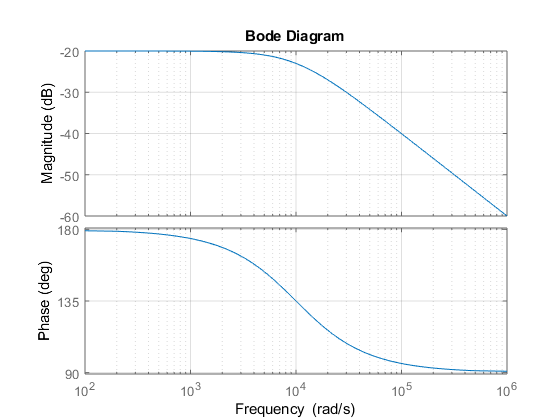
\includegraphics[width=.4\textwidth]{imagens/bode_plot_fig2_2_fty.png}
	\caption{Diagrama de Bode para $R_0$ finito}
	\label{fig:integrador_r0_fin}
\end{figure}

Esse circuito é conhecido como circuito integrador com limitação do ganho em D.C.

Observe que nos cálculos desprezamos o termo k, o qual resultaria na transformada $k=\frac{1}{s}$. A supressão foi feita a partir da hipótese de condição inicial nula. Deixaremos a cargo do leitor a análise do caso em que a condição inicial é não nula.

A inserção de $R_0$ resultou numa estabilidade do circuito antes de encontrarmos o primeiro polo. Note que há uma queda de tensão desde o início. Se quiséssemos uma queda de tensão inicial nula, deveríamos dimensionar $R_0$ para ser idêntico a R.

